\subsection{Designing Statistics Calculator} % (fold)
\label{sub:designing_statistics_calculator}

\tref{tbl:stats-calc-prog} contains a description of a small statistics programs. This program reads a number of values from the user, and then outputs some statistics calculated from these values. This program will make use of arrays to store the values entered, and then calculate the required statistics.

\begin{table}[h]
\centering
\begin{tabular}{l|p{10cm}}
  \hline
  \multicolumn{2}{c}{\textbf{Program Description}} \\
  \hline
  \textbf{Name} & \emph{Statistics Calculator} \\
  \\
  \textbf{Description} & Reads values from the user and calculates a range of statistics that are output to the Terminal. Statistics output include \textbf{mean}, \textbf{maximum}, \textbf{sum}, and \textbf{variance}.\\
  \hline
\end{tabular}
\caption{Description of the Statistics Calculator program.}
\label{tbl:stats-calc-prog}
\end{table}

As before, the process to design and implement this program will follow a number of steps:
\begin{enumerate}
  \item Understand the problem, and get some ideas on the tasks that need to be performed.
  \item Choose the artefacts we will create and use
  \item Design the control flow for the procedural\footnote{The program, and any Functions and Procedures.} artefacts
  \item Map these artefacts to code
  \item Compile and run the program
\end{enumerate}

% subsection designing_statistics_calculator (end)

\subsection{Understanding the Statistics Calculator} % (fold)
\label{sub:understanding_the_statistics_calculator}

Most of the ideas around the Statistics Calculator should be fairly straight forward. The main thing to be checked if the equation needed to calculate the different statistics, and then to convert these into steps for the computer.

\subsubsection{Calculating Sum} % (fold)
\label{ssub:calculating_sum}

The \textbf{sum} is the simplest of the Statistics to calculate. This involves adding together all of the numbers in the array. The main issue here is that the computer cannot add all of these values together, and we must rethink our logic to express it in terms of processing \emph{for each} element.

Think about the way you would sum a list of numbers, this is now the task you need to code for the Computer. What is it that you do with each number? To think this through write a list of random numbers down, and then calculate the sum. Do it slowly, and think about the tasks that you are performing \emph{for each number}.

You should have noticed that you are keeping a running total, and that you add the value of each number from the list to that. When you have done this for each number in the list you have the total. The Pseudocode for this is shown in \lref{plst:sum}.

\pseudocode{plst:sum}{Pseudocode for Sum}{topics/arrays/application/Sum.txt}

\csection{\ccode{clst:sum}{C code for Sum Function. You can read the for loop as \emph{`i starts at 0; while i is less than size; increment i at the end of the loop'}}{topics/arrays/application/sum.c}}

\passection{\pascode{paslst:sum}{Pascal code for Sum Function}{topics/arrays/application/Sum.pas}}

There are three key things to notice about the Pseudocode in \lref{plst:sum}. Firstly the \nameref{sub:for_loop} is used to repeat the loop once for each element in the array. Second, the \texttt{i} variable moves through the valid indexes for the array. Finally, the total is used to keep the running total throughout the code.

The for loop in \nameref{sub:for_loop} will repeat its body once for each value in the array. The \texttt{i} variable will be updated to have the \emph{current} index value each time the loop is repeated. Within the loop the $i^{th}$ value from the array is accessed. This is how the for loop processes each of the values from the array.

The \texttt{total} value keeps track of the current running total. Before the loop its value is set to 0, ensuring that it is appropriately initialised. In the body of the loop the current ($i^{th}$) value of the array is added to the \texttt{total}, and the result stored back into \texttt{total}. This means that by the end of the loop the \texttt{total} variable is now storing the sum of all of the elements of the array.

C and Pascal differ in the amount of support they have for working with arrays. C has very limited support, meaning that you need to do some extra work. Pascal has more build in support for arrays, making some common tasks easier to achieve. The main difference is that C does not keep track of the length of an array. This means that you need to pass the number of elements in the array along with the array to functions and procedures that will work with this data. Pascal, on the other hand, does keep track of the length of arrays and gives you three functions you can use to manage this: \texttt{Low} returns the first index of the array, \texttt{High} returns the last index of the array, \texttt{Length} returns the number of elements in the array.

\csection{The C code for the \texttt{Sum} function is in \lref{clst:sum}. Notice how the \texttt{size} parameter is being used to represent the number of elements in the array. This loop is the standard pattern used to code \nameref{sub:for_loop}s that loop over elements in an array in C.}

\passection{The Pascal code for the \texttt{Sum} function is in \lref{paslst:sum}. Notice how it is using the \texttt{Low} and \texttt{High} functions to get the range of valid array indexes. This loop is the standard pattern used to code \nameref{sub:for_loop}s that loop over elements in an array in Pascal.}

% subsubsection calculating_sum (end)

\clearpage
\subsubsection{Calculating Mean} % (fold)
\label{ssub:calculating_mean}

The mean of a list of values is the sum of those values divided by the number of values. In the case of the Statistics Calculator program there is already a \texttt{Sum} function, so the \texttt{Mean} function does not need to recalculate the sum, it can just call the \texttt{Sum} and use the result returned.

The length of the array can be calculated in Pascal using its \texttt{Length} function, where as C can use the \texttt{size} parameter to determine the number of elements in the array. In both cases the basic logic is the same, you use the \texttt{Sum} function to calculate the sum and then divide this by the number of elements in the array.

\pseudocode{plst:mean}{Pseudocode for Mean}{topics/arrays/application/Mean.txt}

\csection{\ccode{clst:mean}{C code for Mean Function}{topics/arrays/application/mean.c}}

\passection{\pascode{paslst:mean}{Pascal code for Mean Function}{topics/arrays/application/Mean.pas}}

% subsubsection calculating_mean (end)

\clearpage
\subsubsection{Calculating Maximum} % (fold)
\label{ssub:calculating_maximum}

Calculating the largest value in the array, the maximum, will require the logic be adjusted to use the \emph{for each} style. How do you calculate the largest value in a list of numbers? With a small list you are likely to just quickly scan it and see the largest value. Think about the tasks you need to perform, and maybe think about how you would do it for a very long list of numbers, one that spans across many pages.

The algorithm needed to find the maximum value in an array needs to perform an action \emph{for each} element of the array. It needs to process each value in isolation, ignoring the other values from the list.

The key is similar to the logic from the \texttt{Sum} function. You need to keep a \emph{running} maximum. This will store the \emph{current} maximum from the array as you loop through \emph{each element} of the array. Like the sum this value can be updated within the loop.

The Pseudocode for this is in \lref{plst:max}. Notice that its basic layout if the same as the \texttt{Sum} function in \lref{plst:sum}. It initialises the \texttt{max} value and then loops through the array performing an action for each value. In this case the action is to check if the $i^{th}$ value of the array is larger than the running maximum in the \texttt{max} variable. When this is the case a new maximum has been found and is stored in the \texttt{max} variable.

One of the important differences between \texttt{Maximum} and \texttt{Sum} is the initialisation of the \texttt{max} value. In \texttt{Maximum} this cannot be initialised to 0 as this would fail to find the maximum if all values were negative. The maximum must be a value from the array, so it is initialised to the first value in the array. The for loop will then start looping from the $2^{nd}$ element, as the $1^{st}$ has already been processed.

\pseudocode{plst:max}{Pseudocode for Maximum}{topics/arrays/application/Max.txt}

% \csection{\ccode{clst:max}{C code for Maximum Function}{topics/arrays/application/max.c}}
% 
% \passection{\pascode{paslst:max}{Pascal code for Maximum Function}{topics/arrays/application/Max.pas}}

% subsubsection calculating_maximum (end)

\clearpage
\subsubsection{Calculating Variance} % (fold)
\label{ssub:calculating_variance}

The last statistic to calculate is the Variance. The processing for this will be very similar to the \texttt{Sum} and \texttt{Maximum} functions, though the actual calculation is a little more complex. \eref{eq:var} shows how the Variance of a sample is calculated.

\begin{equation}
  \label{eq:var}
  var(x) = \frac{\displaystyle \sum_{i=1}^{n}(x_{i} - \overline{x})^2}{n - 1}
\end{equation}

In \eref{eq:var} $x$ is the array being processed, $\overline{x}$ is the mean of $x$, $x_i$ is the value of the $i^{th}$ element of $x$, and $n$ is the number of elements in the array. The Sigma indicates that $x_{i} - \overline{x}$ needs to be summed for each element of $x$.

The steps to calculate the Variance are therefore:
\begin{enumerate}
  \item Determine the value of the mean ($\overline{x}$).
  \item Calculate $(x_{i} - \overline{x})^2$ for each element, and store these in a running sum (called \texttt{temp}).
  \item Divide the value (from \texttt{temp}) by the number of elements in the array minus one.
\end{enumerate}

The matching Pseudocode for this is shown in \lref{plst:variance}. In this case $x$ is the \texttt{data} array. In Step 1 the mean ($\overline{x}$) is calculated once and stored in \texttt{avg}. The loop starts at Step 3, and runs \emph{for each} element of the array. The value $(x_{i} - \overline{x})^2$ is calculated for each element in Step 4, and added to the running total stored in \texttt{temp}. The final result is then calculated and the result returned in Step 5.

\pseudocode{plst:variance}{Pseudocode for Variance}{topics/arrays/application/Variance.txt}

% subsubsection calculating_variance (end)

% subsection understanding_the_statistics_calculator (end)

\clearpage
\subsection{Choosing Artefacts for Statistics Calculator} % (fold)
\label{sub:choosing_artefacts_for_statistics_calculator}

In understanding these concepts we have uncovered some Functions that will be included in the program's design. 

With the calculations thought through the design seems to be coming together. So far we have thought through the steps needed to calculate the output, but we have not thought about how these values will be read into the program.

Programs can be thought of as transforming data, taking inputs and generating outputs, as shown in \fref{fig:input-output-overview}. So far we have examined the processing needed to create the outputs, but we still need to consider how the data gets into the program, the inputs.

\begin{figure}[h]
   \centering
   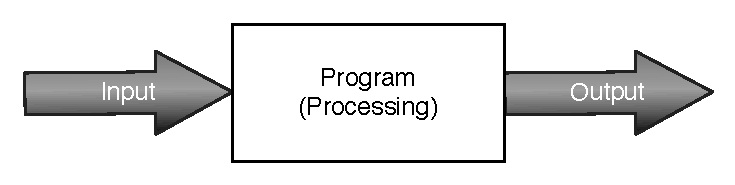
\includegraphics[width=0.6\textwidth]{./topics/arrays/diagrams/ProcessingOverview} 
   \caption{Programs convert Inputs to Outputs}
   \label{fig:input-output-overview}
\end{figure}

At the start of the program the user will need to enter the values that will be stored in the array. This task can be coded in a \texttt{Populate Array} procedure. This will get the user to enter all of the values into the array. In other words it will allow the user to enter \emph{each value} in the array.

The logic for populating the array can be split into a \texttt{Populate Array} procedure that calls a \texttt{Read Double} function. The \texttt{Read Double} function will be very useful across a number of different programs, so this may be able to be used elsewhere.

\subsubsection{Reading double values from the user} % (fold)
\label{ssub:reading_double_values_from_the_user}

\fref{fig:read-double-flow} shows the flowchart for the process of reading a double value from the user. This includes a \nameref{sub:pre_test_loop} that repeatedly asks the user to enter a number if they value they enter is not a number. This demonstrates a standard \emph{validation} loop, in which you read a value, and check that it is valid in a loop. 

The C and Pascal code for this are both slightly different to the flowchart due to different way they handle input and the features they offer to for converting the value read to a number. Details of these are shown alongside \lref{clst:read_double} and \lref{paslst:read_double}.

\begin{figure}[htbp]
   \centering
   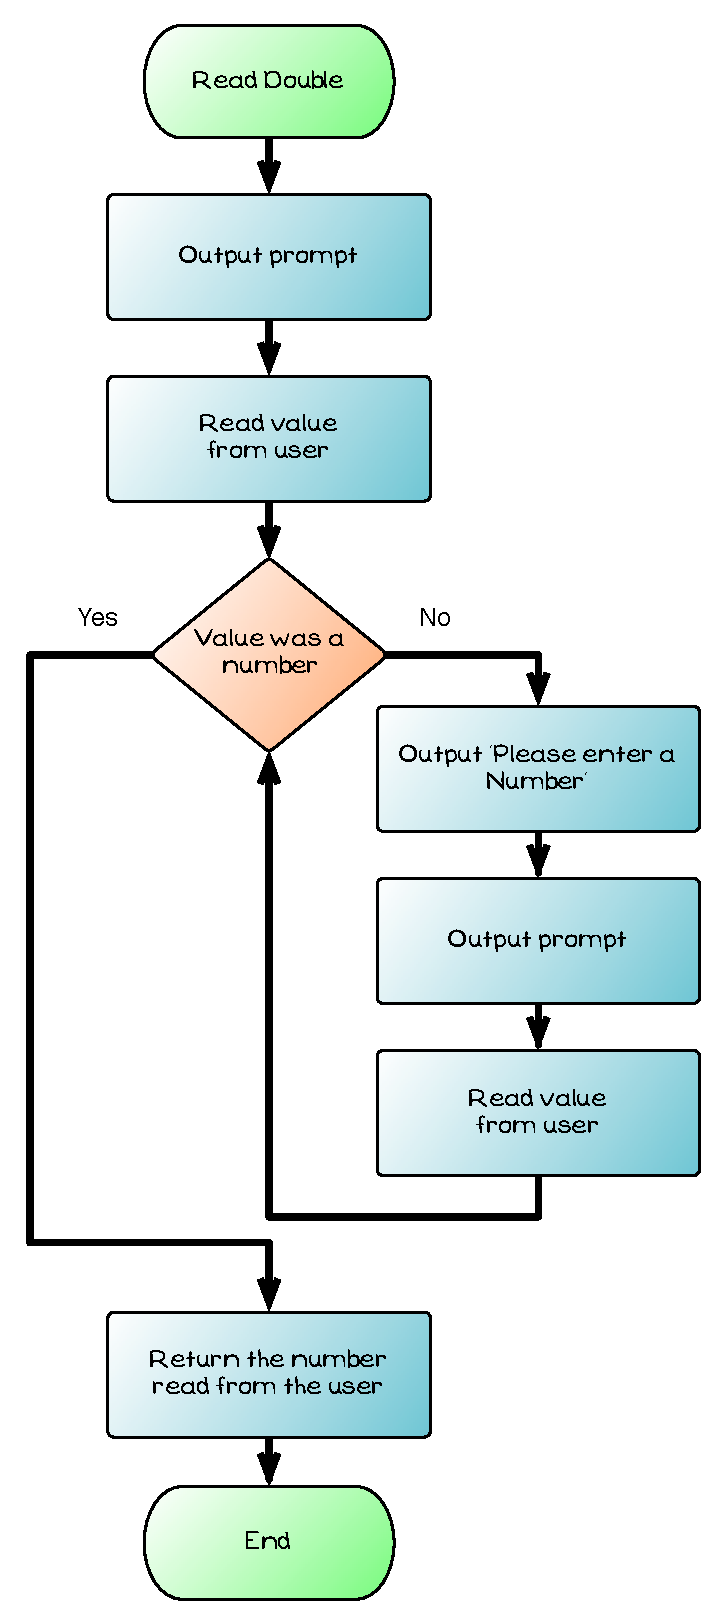
\includegraphics[width=0.45\textwidth]{./topics/arrays/diagrams/ReadDouble} 
   \caption{Flowchart showing the process for reading a double}
   \label{fig:read-double-flow}
\end{figure}

\clearpage

\csection{The C version of \texttt{Read Double}, shown in \lref{clst:read_double}, uses \texttt{scanf} (see \nameref{sub:c_terminal_input}) to read and format the number in the one action. The \texttt{scanf} Function returns a value indicating the number of conversions that were successful. This can be checked in the loop, and the loop is repeated \emph{while} \texttt{scanf} did not convert one value.
\newline\newline
In the loop itself the \texttt{scanf} is used to read past the value that is not a number, as \texttt{scanf} does not proceed when it finds an error. The format string in \texttt{scanf} indicates that it should read everything up to the end of the line.
\ccode{clst:read_double}{C code for \texttt{Read Double}}{topics/arrays/application/read-double.c}}

\passection{The Pascal version of \texttt{Read Double}, shown in \lref{paslst:read_double}, reads the input as a string and then try to convert it to a double. The \texttt{TryStrToInt} Function attempts to convert the text read into a number, storing the value in the \emph{result} variable.
\pascode{paslst:read_double}{Pascal code for \texttt{Read Double}}{topics/arrays/application/ReadDouble.pas}}

% subsubsection reading_double_values_from_the_user (end)

\clearpage
\subsubsection{Populating the Array} % (fold)
\label{ssub:populating_the_array}

With the logic for \texttt{Read Double} in place the next step is to determine the steps needed in the \texttt{Populate Array} procedure. This procedure will loop and read a value from the user for each element of the array. This can use the \texttt{Read Double} function to get the value from the user, and then store this in the array's elements.

A flowchart illustrating the steps in \texttt{Populate Array} is shown in \fref{fig:populate-array-flow}. The decision node is being used to show the control mechanism of the for loop, counting from the lowest index of the array to the highest index. Within the body of the loop the two instructions build a prompt string, and then use this in the call to \texttt{Read Double}. The result returned from \texttt{Read Double} is stored in the current ($i^{th}$) element of the array.

Once again the C and Pascal code differ in how this is implemented, centred on how the \emph{prompt} is built within the loop. Pascal has built in support for Strings, so its code is much simpler. The C code for this requires you to coordinate the steps needed to build the text for the prompt. The details for these are shown in the text accompanying \lref{clst:populate_array} and \lref{paslst:populate_array}.

\begin{figure}[htbp]
   \centering
   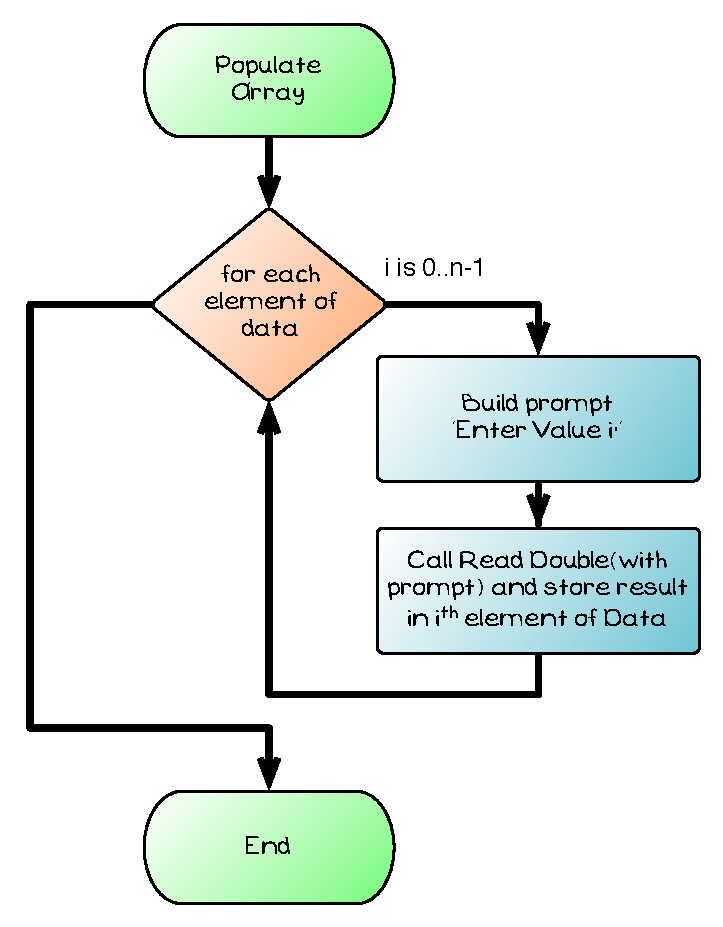
\includegraphics[width=0.6\textwidth]{./topics/arrays/diagrams/PopulateArray} 
   \caption{Flowchart showing the process for \texttt{Populate Array}}
   \label{fig:populate-array-flow}
\end{figure}

\begin{figure}[htbp]
\csection{The C version of \texttt{Populate Array} is shown in \lref{clst:populate_array}. This uses the following functions from \texttt{strings.h}. As C does not know the length of the string each of these functions takes a number (\texttt{n}) that indicates the maximum number of characters to copy.
\begin{itemize}
  \item \texttt{\textbf{strncpy}}: String Copy (n characters). The first parameter is the destination, the second the source, the third is the number of characters.
  \item \texttt{\textbf{sprintf}}: Same as \texttt{printf} (see \nameref{sub:c_console_output}), except that the output is stored in a c-string. In this case the \csnipet{"\% 100"} ensures that only 2 characters (plus the terminator) are written into the string. See \sref{sub:c_string} \nameref{sub:c_string}.
  \item \textbf{\texttt{strncat}}: String Concatenate (n characters). Adds the text in parameter 2 to the end of the string in parameter 1. 
\end{itemize}

\ccode{clst:populate_array}{C code for \texttt{Populate Array}}{topics/arrays/application/populate-array.c}}  
\end{figure}

\begin{figure}[htbp]
  \passection{The Pascal version of \texttt{Populate Array} is shown in \lref{paslst:populate_array}. This uses Pascal's \textbf{\texttt{IntToStr}} function to convert the value \texttt{i + 1} from Integer to String.
  \pascode{paslst:populate_array}{Pascal code for \texttt{Populate Array}}{topics/arrays/application/PopulateArray.pas}}  
\end{figure}

% subsubsection populating_the_array (end)

\subsubsection{Where is the data stored} % (fold)
\label{ssub:where_is_the_data_stored}

The last question to remain is where will the data be stored. The array is a kind of variable, and therefore the array could be a \nameref{sub:local_variable} or a \nameref{sub:global_variable}. As Global Variables should be avoided where possible, this will be coded as a \textbf{Local Variable} within the program's \texttt{Main} procedure. It can then be passed from there to the other Functions and Procedures in the code.

% subsubsection where_is_the_data_stored (end)

\clearpage
\subsubsection{Overview of Statistics Calculator's design} % (fold)
\label{ssub:overview_of_statistics_calculators_design}

That completes the logic needed to implement the Statistics Calculator Program. The final structure is shown in \fref{fig:stats-calc-struct} as a Structure Chart. Notice the double headed arrow on \texttt{data} in the call from \texttt{Main} to \texttt{Populate Array}. This indicates that the data parameter is passing the values into, and getting values out of the \texttt{Populate Array} procedure. Also see how the \texttt{data} value is passed out of \texttt{Main} to the functions that calculate the statistics.

\begin{figure}[htbp]
   \centering
   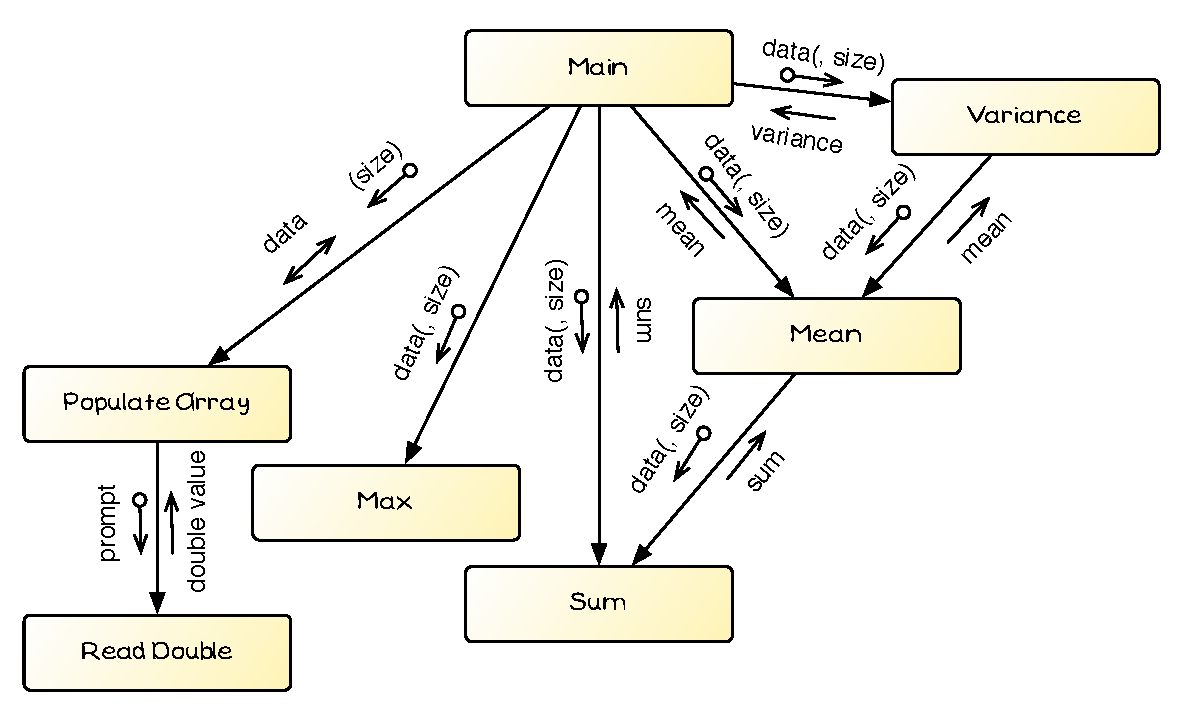
\includegraphics[width=\textwidth]{./topics/arrays/diagrams/StatsCalcStruct} 
   \caption{Structure Chart showing the structure of the \texttt{Statistics Calculator} program}
   \label{fig:stats-calc-struct}
\end{figure}

\mynote{
\begin{itemize}
  \item Remember anytime you need to do something with all of the elements in an array you need to work out how you can achieve this \textbf{for each} element in the array.
  \item Notice that the processing of individual value from the arrays are always similar.
  \item Make sure you can see how the for loop is able to perform these values for each element of the array.
\end{itemize}
}

% subsubsection overview_of_statistics_calculators_design (end)
% subsection choosing_artefacts_for_statistics_calculator (end)

\subsection{Writing the Code for Statistics Calculator} % (fold)
\label{sub:writing_the_code_for_statistics_calculator}

The flowcharts and Pseudocode shown communicate the logic that needs to be coded into the Functions and Procedures of this program. The following two sections, \sref{sec:arrays_in_c} \nameref{sec:arrays_in_c} and  \sref{sec:arrays_in_pascal} \nameref{sec:arrays_in_pascal}, contain a description of the syntax needed to code arrays in the C and Pascal programming languages. This information can be used to write the code for the Statistics Calculator, and other programs.

% subsection writing_the_code_for_statistics_calculator (end)
\clearpage
\subsection{Compiling and Running Statistics Calculator} % (fold)
\label{sub:compiling_and_running_statistics_calculator}

When the code is finished you can compile and run the program. It is a good idea to implement the solution a little bit at a time, compiling and running it frequently as you progress. Try implementing the solution using the following smaller steps, and the tests shown for each.

\begin{enumerate}
  \item Start by getting \texttt{Read Double} to work. In \texttt{Main} just read a single value and output it to the Terminal. \textbf{Tests}:
  \begin{itemize}
    \item Check that a number can be read correctly.
    \item Try entering text, and check the error message is shown and that you can enter a number the next time.
    \item Try entering multiple text values on a single line.
    \item Try entering multiple text values, one after the other.
  \end{itemize}
  \item Implement \texttt{Populate Array}. Include an array in \texttt{Main}, and have its values read in by \texttt{Populate Array}. Print the values back to the Terminal so that you can check this code is working. \textbf{Tests}:
  \begin{itemize}
    \item Enter each of the values and check they are printed out correctly.
    \item Try entering text, this should be handled by \texttt{Read Double} but check it is working correctly with \texttt{Populate Array}.
  \end{itemize}
  \item Implement the \texttt{Sum} Function.
  \textbf{Tests}:
  \begin{itemize}
    \item Test that it works with some basic values.
    \item Try all negative values.
    \item Try a mix of positive and negative values.
  \end{itemize}
  \item Implement the \texttt{Mean} Function. Same tests as \texttt{Sum}.
  \item Implement the \texttt{Variance} Function. Same tests as \texttt{Sum}.
  \item Finish by implementing the \texttt{Maximum} Function. Same tests as \texttt{Sum}.
\end{enumerate}

By building the code a little at a time, and running tests as you go, you will have less code to search when you do find an issue. This makes it easier to fix those little errors that are likely to slip into the code from time to time.

When this iterative process is complete you should have a solution for the Statistics Calculator. You should be able to easily change this so that it can read in ten, a hundred, or even a thousand values from the user. This is something that would not have been possible without using arrays.

\mynote{
\begin{itemize}
  \item Get your code running as soon as you can.
  \item Build a little and test a little as you go.
  \item When you find a bug start looking for it in the code you just added (or changed).
  \item You can perform this as a \emph{\textbf{design, implement, compile, test}} cycle. This enables you to build the program a small piece at a time. Before you start this it is likely to be a good idea to have at least a sketched out plan for the design.
  \item As you develop your design skills you will be able to create larger designs before you code. While you are learning to program it is ok to design and code at the same time as this lets you to quickly test if your design will work.
\end{itemize}
}

% subsection compiling_and_running_statistics_calculator (end)
